% !TEX program = xelatex

\documentclass{article}
\usepackage[T1]{fontenc}
\usepackage{fontspec}
\usepackage{lmodern}
\usepackage[czech]{babel}
\usepackage[top = 1.5cm, bottom = 1.5cm, left = 2cm, right = 2cm]{geometry}
\usepackage{amsmath}
\usepackage{amssymb}
\usepackage{mathtools}
\usepackage{letltxmacro}
\usepackage{wrapfig}
\usepackage{bbm}
\usepackage{csquotes}
\usepackage{nicefrac}
\usepackage{hyperref}

\usepackage{gnuplottex}


% import obrázků z Inkscape
% podle návodu na https://castel.dev/post/lecture-notes-2/
\usepackage{import}
\usepackage{xifthen}
\usepackage{pdfpages}
\usepackage{transparent}

\newcommand{\incfig}[1]{%
    \def\svgwidth{\columnwidth}
    \import{./}{#1.pdf_tex}
}


\LetLtxMacro{\oldhbar}{\hbar}
\renewcommand*{\hbar}{{\mathpalette\hbaraux\relax\mathrm{h}}}
\newcommand*{\hbaraux}[2]{\sbox0{\mathsurround=0pt$#1\mathchar'26$}\mkern-1mu\lower.07\ht0\box0\mkern-8mu}

\newcommand\kludgequote[1]{%
    \prescript {} {\text{\normalsize„}} {\mkern-1.5mu#1} 
    {\vphantom{#1}}^{\mkern-1.5mu\text{\normalsize\raisebox{-0.5ex}{“}}}}

\def\ph{\phantom}
\def\vph{\vphantom}
\def\hph{\hphantom}
\def\rzw{\mathrlap}
\def\lzw{\mathllap}
\def\czw{\mathclap}

\newcommand{\comm}[2]{\left[ #1, #2 \right]}
\newcommand{\const}[1]{\text{#1}}
\newcommand{\norm}[1]{\left\lVert#1\right\rVert}
\newcommand{\innerprod}[2]{\big< #1, #2 \big>}
\newcommand{\mean}[1]{\big< #1 \big>}
\renewcommand{\d}[1]{\;\const{d}#1}
\newcommand{\dd}[2]{\frac{\const{d} #1}{\const{d} #2} \;}
\newcommand{\pd}[2]{\frac{\partial  #1}{\partial  #2} \;}
\newcommand{\e}[1]{\const{e}^{#1}}
\renewcommand{\i}{\const{i}}
\newcommand{\bhat}[1]{\hat{\bm{#1}}}
\newcommand{\vechat}[1]{\hat{\vec{#1}}}
\renewcommand{\dot}[1]{\accentset{\bullet}{#1}}
\newcommand{\Tr}{\operatorname{Tr}}
\newcommand{\bra}[1]{\left< #1 \right|}
\newcommand{\ket}[1]{\left| #1 \right>}
\newcommand{\braket}[2]{\left< #1 \middle| #2 \right>}
\newcommand{\f}{\varphi}
\newcommand{\Parity}{\hat{\mathcal{P}}}
\newcommand{\R}{\mathbb{R}}
\renewcommand{\C}{\mathbb{C}}

\newcommand{\mat}[1]{
    \begin{pmatrix}
        #1
    \end{pmatrix}
}

\newcommand{\mata}[2]{
    \left(
    \begin{array}{@{}#1@{}}
        #2
    \end{array}
    \right)
}

\newcommand{\smat}[2][1]{
    \scalebox{#1}{$\mat{#2}$}
}

\begin{document}

\section*{Úkol 4: Potenciálový schod s delta jámou}
\textbf{Autor: Michal Grňo}

\subsection*{Zadání}
Na $L^2(\R)$ máme zadaný hamiltonián
\begin{align*}
    \hat H =
    - \frac{\hbar^2}{2m} \, \dd{^2}{x^2}
    + V_0 \, \theta(x)
    - \lambda \, \delta(x)
    \: ,
\end{align*}
kde $\theta(x)$ je Heavisidova funkce. Přejděte k bezrozměrným veličinám $q=x/x_0$, $\epsilon=E/V_0$. Najděte podmínku pro existenci vázaného stavu. Jaká je pravděpodobnost, že se v takovém stavu zachytí elektron popsaný vlnovou funkcí $\exp(-\alpha|x|)$, $\alpha>0$?

\subsection*{Řešení}
\subsubsection*{Interpretace zadání}
Nejprve je vhodné ujasnit si, co vlastně výraz z matematického hlediska znamená. Celý hamiltonián je endomorfismem na $L^2$, jeho jednotlivé sčítance ovšem nutně nemusí být. Konkrétně nemá smysl vyžadovat od operátoru „násobení delta funkcí“, aby byl zobrazením $L^2 \to L^2$, jeho definičním oborem by totiž musely být funkce, které jsou nulové na okolí nuly, a akce takového operátoru by byla nutně (a nudně) triviální. Místo toho si obor hodnot jednotlivých sčítanců vhodně rozšíříme na distribuce $\mathcal{D}'$ a až po součtu budeme vyžadovat, aby byl z $L^2 \subset \mathcal{D}'$.
\begin{gather*}
    \hat \partial^2 = \kludgequote{ \dd{^2}{x^2} \!\! } \\[3pt]
    \hat \partial^2 : L^2(\R) \to \mathcal{D}'(\R) \\[1pt]
    \left< \hat \partial^2 f, \; \varphi \right>
    \coloneqq \int_\R f(x) \, \varphi''(x) \d{x}
    \quad \forall f \in L^2(\R) \; \forall \varphi \in \mathcal{D}(\R)
\end{gather*}

\begin{gather*}
    \hat \theta: L^2(\R) \to L^2(\R) \\[2pt]
    \hat \theta f = x \mapsto \theta(x) \, f(x)
\end{gather*}

\begin{gather*}
    \hat\delta = \kludgequote{ \delta(x) } \\[3pt]
    \hat\delta: {\rm D}(\hat\delta) \to \mathcal{D}' \\[2pt]
    {\rm D}(\hat\delta) = \{ \; f \in L^2(\R) \;|\; f \text{ je spojitá na okolí nuly} \; \} \\[2pt]
    \left< \hat\delta f, \varphi \right>
    \coloneqq \left< \vph{\hat\delta} f(0) \, \delta, \varphi \right>
    = f(0) \, \varphi(0)
    \quad \forall f \in {\rm D}(\hat\delta) \; \forall \varphi \in \mathcal{D}(\R)
    \\
\end{gather*}
Pozornému čtenáři jistě neuniklo, že předchozí sada výrazů vypadá jako detektiv v klobouku. 

\subsubsection*{Přechod k bezrozměrnému operátoru}
Nyní bychom chtěli od výrazu s fyzikálními jednotkami přejít k bezrozměrnému, čistě „matematickému“ operátoru. Začneme transformací souřadnic $\rho(q) \coloneqq x_0 \, q = x$. Chceme, aby operátory „komutovaly“ s transformací, tj. aby platilo:
\begin{align*}
    \hat A' f' = (\hat A f)' \: ,
    \qquad
    \text{kde } f' \coloneqq f \circ \rho \: .
\end{align*}
(V předchozím řádku výjimečně $f'$ neznamená derivaci.) Proto se všechny operátory musí transformovat
\begin{align*}
    \hat A(f) \quad \mapsto \quad \hat A(f \circ \rho^{-1}) \circ \rho \: .
\end{align*}
Také se nám bude hodit vztah pro pull-back distribuce:
\begin{align*}
    \left<T \circ \rho, \; \varphi \right> = \left<T, \; \frac{\varphi \circ \rho^{-1}}{|\rho' \circ \rho^{-1}|} \right> \: .
\end{align*}
\pagebreak

\noindent
Tyto dva vzorečky aplikujeme postupně na všechny operátory v zadání hamiltoniánu:
\begin{gather*}
    \left< \hat \partial^2(f \circ \rho^{-1}) \circ \rho, \; \varphi \right> =
    \left< \hat \partial^2(f \circ \rho^{-1}), \; \frac{1}{x_0} \, \varphi \circ \rho^{-1} \right> =
    \left< f \circ \rho^{-1}, \; \frac{1}{{x_0}^3} \, \varphi'' \circ \rho^{-1} \right> =
    \left< f, \; \frac{1}{{x_0}^2} \, \varphi'' \right> =
    \left< \frac{1}{{x_0}^2} \; \hat \partial^2 \, f, \; \varphi \right>
    \\\\
    \left<\hat \theta (f \circ \rho^{-1}) \circ \rho, \; \varphi \right> =
    \left<\hat \theta (f \circ \rho^{-1}), \; \frac{1}{x_0} \, \varphi \circ \rho^{-1} \right> =
    \left<f \circ \rho^{-1} \!, \; \frac{1}{x_0} \, (\varphi \circ \rho^{-1}) \, \theta \right> =
    \left<f, \; (\theta \circ \rho) \varphi \right> =
    \left<f, \; \theta \, \varphi \right> =
    \left<\hat \theta f, \; \varphi \right>
    \\\\
    \left<\hat \delta (f \circ \rho^{-1}) \circ \rho, \; \varphi \right> =
    \left<\hat \delta (f \circ \rho^{-1}), \; \frac{1}{x_0} \, \varphi  \circ \rho^{-1}\right> =
    \left<\delta , \; \frac{1}{x_0} \, (\varphi  \circ \rho^{-1}) \, (f \circ \rho^{-1})\right> =
    \frac{1}{x_0} \, \varphi(0) \, f(0) =
    \left< \frac{1}{x_0} \, \hat \delta f, \; \varphi \right>
\end{gather*}
Po transformaci souřadnic tedy máme
\begin{align*}
    \hat\partial^2 &\mapsto \frac{1}{{x_0}^2} \, \hat\partial^2 \: , &
    \hat\theta &\mapsto \hat\theta \: , &
    \hat\delta &\mapsto \frac{1}{x_0} \, \hat\delta \: .
\end{align*}
\begin{align*}
    \hat H_{\rm trans.} =
    - \frac{\hbar^2}{2m {x_0}^2} \, \hat\partial^2
    + V_0 \, \hat\theta
    - \frac{\lambda}{x_0} \, \hat\delta
    \: .
\end{align*}
Ještě potřebujeme přejít od energie k bezrozměrné veličině $\epsilon = E/V_0$. Tento přechod bude významně snazší – protože rozměr energie má samotný hamiltonián, stačí celý výraz vydělit skalárem $V_0$:
\begin{align*}
    \frac{1}{V_0} \, \hat H_{\rm trans.} =
    - \frac{\hbar^2}{2 \, m \, {x_0}^2 \, V_0} \, \hat\partial^2
    + \hat\theta
    - \frac{\lambda}{x_0 \, V_0} \, \hat\delta
    \: .
\end{align*}
Zavedeme si zkratku $a=\lambda / x_0 V_0$. Jelikož máme volnost zvolit si za $x_0$ jakoukoliv hodnotu s rozměrem délky, zvolíme
\begin{align*}
    x_0 = \frac{\hbar}{\sqrt{2 \, m \, V_0}} \: ,
\end{align*}
čímž dostáváme výrazně jednodušší, bezrozměrný tvar hamiltoniánu:
\begin{align*}
    \hat L = - \hat\partial^2 + \hat\theta - a \, \hat\delta \: .
\end{align*}

\subsubsection*{Definiční obor a samosdruženost}
Nyní je načase zamyslet se nad definičním oborem operátoru $\hat L$. Nejprve se podíváme na přirozené definiční obory a obory hodnot jednotlivých sčítanců. Operátor $\hat\delta$ zobrazuje z funkcí spojitých na okolí nuly na násobky $\delta$ v nule:
\begin{align*}
    \hat\delta \, (f \in L^2 \cap \mathcal{C}_{\{0\}}) = f(0) \, \delta
\end{align*}
Operátor $\hat\theta$ násobení Heavisidovou funkcí zobrazuje funkce z $L^2$ zpět do $L^2$. Oproti tomu slabá derivace $\hat\partial$ má na $L^2$ mnohem větší obor hodnot – slabá derivace $\hat\partial^2$ funkce $f \in L^2$ může vyjít jako jakákoliv regulární distribuce (tj. lokálně integrovatelná funkce) plus delty a jejich první derivace v bodech, kde mají $f$ a $f'$ skokové nespojitosti.
\begin{align*}
    \hat\partial^2 \, (f \in L^2) =
    (g \in L^1_{\rm loc}) + \sum_j \alpha_j \; \delta(q - q_j) + \sum_k \beta_j \; \delta'(q - q_k)
\end{align*}
Chceme-li, aby obor hodnot $\hat\partial^2 - a \hat\delta$ ležel v $L^2$, musíme omezit definiční obor. Budeme-li požadovat, aby $f$ byla ze Sobolevova prostoru $W^{1,2}(\R) \subset L^2(\R)$, zbavíme se derivací delt a zařídíme, aby $f'' \in L^2$. Navíc můžeme požadovat, aby $f \in W^{2,2}(\R \setminus \{0\})$, čímž dostaneme:
\begin{align*}
    (\hat\partial^2 + a \hat\delta) f
    = (f'' \in L^2)
    + \big( f'(0+) - f'(0-) \big) \delta
    + a \delta
\end{align*}
Nakonec budeme požadovat, aby $f'(0+)-f'(0-) = -a \, f(0)$, čímž implicitně také požadujeme, aby limity $f'(0+)$ a $f'(0-)$ existovaly . To, že $f$ je na okolí nuly spojitá a výraz $f(0)$ má tedy dobrý smysl, máme zaručeno z příslušnosti do $W^{1,2}$. Tím dostaneme konečně funkci z $L^2$. Maximální \textit{„přirozený“} definiční obor operátoru $\hat L$ je tedy:
\begin{align*}
    {\rm D}(\hat L) = 
    \big\{\;
        f \in W^{1,2}(\R) \;\cap\; W^{2,2}(\R \setminus \{0\})
    \quad\big|\quad
        f'(0+) - f'(0-) = -a \, f(0)
    \;\big\}
\end{align*}
V předchozím textu $f'$ a $f''$ samozřejmě značí běžnou derivaci funkce (definovanou skoro všude), ne distribuční derivaci, kterou budeme značit výhradně $\hat\partial f$ a $\hat\partial^2 f$. Maximálním „přirozeným“ definičním oborem myslíme takový, na kterém platí vzoreček $\hat L = -\hat\partial^2 + \hat\theta - a\hat\delta$ ve významu, v jakém bychom běžně očekávali – tj. distribuční derivace, násobení Heavisidem, násobení delta distribucí. Definiční obor celého $\hat L$ je samozřejmě možné rozšířit, kdybychom to ovšem chtěli udělat, museli bychom dát pozor, zda taková rozšíření budou jednoznačná, v opačném případě bychom si „upravovali zadání“ úlohy a mohli bychom dospět k jiným výsledkům. Uvidíme ale, že žádné rozšiřování definičního oboru nebude potřeba.

Pro funkce z ${\rm D}(\hat L)$ tedy platí tato identita:
\begin{samepage}
\begin{align*}
    (\hat\partial^2 + a\hat\delta) \, f = f''
\end{align*}
Dokonce z teorie distribucí víme, že pro funkce z $L^2$ tato identita platí \textit{právě tehdy}, jsou-li z ${\rm D}(\hat L)$.
\end{samepage}

Pozorovatelné v kvantové mechanice jsou představovány samosdruženými operátory. Kdyby náš operátor $\hat L$ nebyl samosdružený, nemusí to ještě nutně být problém, může mít nějaké samosdružené rozšíření. Stačí nám, aby byl symetrický – tedy musí platit ${\rm D}(\hat L) \subseteq {\rm D}(\hat L^+)$ a $\hat L \psi = \hat L^+ \psi$ pro všechny $\psi$ z ${\rm D}(\hat L)$. Vyšetříme tedy symetrii $\hat L$ a definiční obor $\hat L^+$:
\begin{align*}
    \big( \hat L \, f, \;\; g \big)_{L^2(\R)}
    &= \big( (-\hat\partial^2 + \hat\theta - a\hat\delta) \, f, \;\; g \big)_{L^2(\R)} \\[5pt]
    &= \big( \hat\theta \, f, \;\; g \big)_{L^2(\R)}
    - \big( (\hat\partial^2 + a\hat\delta) \, f, \;\; g \big)_{L^2(\R)} \\[5pt]
    &= \big( f, \;\; \hat\theta \, g \big)_{L^2(\R)}
    - \big( f'' \!, \;\; g \big)_{L^2(\R)}
\end{align*}
Nyní bychom chtěli provést integraci \textit{per partes}, to ovšem nemůžeme pro každé $g\in L^2$. Konkrétně, abychom mohli provést \textit{per partes} alespoň po částech intervalu $(-\infty, +\infty)$, musí $g$ a $g'$ být alespoň po částech absolutně spojité. V~případě $f$ a $f'$ nám absolutní spojitost zařizuje příslušnost k $W^{1,2}$ a $W^{2,2}$. Pro pohodlnost budeme nejprve předpokládat, že $g \in {\rm D}(\hat L)$, a teprve dodatečně budeme diskutovat, zda nemůžeme použít $g$ obecnější. Explicitně to pro $g$ znamená, že:
\begin{equation*}
    g \in W^{1,2}(\R) \;\cap\; W^{2,2}(\R \setminus \{0\})
    \: , \qquad
    g'(0+) - g'(0-) = a \, g(0)
    \: .
\end{equation*}
V takovém případě můžeme spočítat \textit{per partes} následujícím způsobem:
\begin{align*}
    \big( f'', \;\; g \big)_{L^2(\R)}
    &= \int_{-\infty}^{+\infty} \overline f'' g
    = \big[ \, \overline f' g \big]_{-\infty}^{0}
    + \big[ \, \overline f' g \big]_{0}^{+\infty}
    - \int_{-\infty}^{+\infty} \overline f' g' \\[5pt]
    &= \big[ \, \overline f' g \big]_{-\infty}^{+\infty}
    + \overline f'\!(0-) \, g(0-) - \overline f'\!(0+) \, g(0+)
    - \int_{-\infty}^{+\infty} \overline f' g' \\[5pt]
    &= \big[ \, \overline f' g \big]_{-\infty}^{+\infty}
    + \Big( \overline f'(0-) - \overline f'(0+) \Big) \, g(0)
    - \int_{-\infty}^{+\infty} \overline f' g' \\[5pt]
    &= \big[ \, \overline f' g \big]_{-\infty}^{+\infty}
    + a \, f(0) \, g(0)
    - \int_{-\infty}^{+\infty} \overline f' g' \\[5pt]
    &= \big[ \, \overline f' g \big]_{-\infty}^{+\infty}
    + a \, f(0) \, g(0)
    - \big[ \, \overline f \, g' \big]_{-\infty}^{0}
    - \big[ \, \overline f \, g' \big]_{0}^{+\infty}
    + \int_{-\infty}^{+\infty} \overline f g'' \\[5pt]
    &= \big[ \, \overline f' g \big]_{-\infty}^{+\infty}
    + a \, f(0) \, g(0)
    + \Big( \overline g'(0+) - \overline g'(0-) \Big) \, f(0)
    - \big[ \, \overline f \, g' \big]_{-\infty}^{+\infty}
    + \int_{-\infty}^{+\infty} \overline f g'' \\[5pt]
    &= \big[ \, \overline f' g \big]_{-\infty}^{+\infty}
    + a \, f(0) \, g(0)
    - a \, g(0) \, f(0)
    - \big[ \, \overline f \, g' \big]_{-\infty}^{+\infty}
    + \int_{-\infty}^{+\infty} \overline f g'' \\[5pt]
    &= \big[ \, \overline f' g \big]_{-\infty}^{+\infty}
    - \big[ \, \overline f \, g' \big]_{-\infty}^{+\infty}
    + \big( f, \;\; g'' \big)_{L^2(\R)}
\end{align*}
Vidíme, že \textit{obecnější} $g$ povolit nemůžeme, jinak by nám zbyly členy typu $\big(g(c-) - g(c+)\big) \, f(c)$. Nakonec chceme, aby platilo:
\begin{equation*}
    \big[ \, \overline f' g \big]_{-\infty}^{+\infty}
    = \big[ \, \overline f \, g' \big]_{-\infty}^{+\infty}
    = 0
    \qquad \forall f \in {\rm D}(\hat L)
    \label{eq:okrajove-podminky}
\end{equation*}
To máme ale zaručeno\footnote{Pro důkaz viz \url{https://physics.stackexchange.com/q/438009}} z příslušnosti k prostorům $W^{1,2}, \; W^{2,2}$.

\medskip\pagebreak

\noindent
Celkem máme:
\begin{equation*}
    \big( \hat L \, f, \;\; g \big)_{L^2}
    = \big( \hat\theta \, f, \;\; g \big)_{L^2}
    - \big( f'' \!, \;\; g \big)_{L^2}
    = \big( f, \;\; \hat\theta \, g \big)_{L^2}
    - \big( f \!, \;\; g'' \big)_{L^2}
    = \big( f, \;\; \hat L \, g \big)_{L^2}
    \equiv \big( f, \;\; \hat L^+ \, g \big)_{L^2}
\end{equation*}
Ověřili jsme tedy, že operátor
\begin{gather*}
    \hat L = - \hat\partial^2 + \hat\theta - a \, \hat\delta \: ,
    \\
    {\rm D}(\hat L) = 
    \big\{\;
        f \in W^{1,2}(\R) \;\cap\; W^{2,2}(\R \setminus \{0\})
    \quad\big|\quad
        f'(0+) - f'(0-) = -a \, f(0)
    \;\big\}
\end{gather*}
je samosdružený operátor na $L^2(\R)$. Nyní nás zajímá, zda má nějaké bodové spektrum – tedy jestli má nějakou vlastní funkci (tzv. vázaný stav).

\subsubsection*{Vázaný stav}
Budeme hledat normalizovanou vlastní funkci operátoru $\hat L$. Úlohu budeme řešit explicitně jako obyčejnou diferenciální rovnici:
\begin{gather*}
    \hat L \, f = \epsilon \, f \: ,
    \qquad
    f \in {\rm D}(\hat L)
    \\[10pt]
    f'' + \theta \, f = \epsilon \, f
    \\[5pt]
    f'' + (\theta - \epsilon) \, f = 0
\end{gather*}
Kvůli tvaru definičního oboru a přítomnosti Heavisidovy funkce je výhodné řešit rovnici na zvlášť na intervalech $(-\infty, 0)$ a $(0, +\infty)$ a řešení potom „slepit“.
\begin{gather*}
    f_-'' \; - \; \epsilon \, f_- = 0
    \qquad
    f_+'' \; + \; (1-\epsilon) \, f_+ = 0
    \\[5pt]
    f_-(0-) = f_+(0+) \eqqcolon f(0)
    \\[5pt]
    f_-'(0-) - f_+'(0+) = a \, f(0)
\end{gather*}
Bez zohlednění definičního oboru a slepovacích podmínek dostáváme řešení:
\begin{gather*}
    f_-(q) = A \, \e{-\sqrt{-\epsilon \,} \, q} + B \, \e{+\sqrt{-\epsilon \,} \, q}
    \: , \qquad
    f_+(q) = C \, \e{-\sqrt{1-\epsilon \,} \, q} + D \, \e{+\sqrt{1-\epsilon \,} \, q}
\end{gather*}
Všechna tato řešení jsou kandidáty na slabé vlastní funkce ve smyslu $\big<T,\, \hat L \, \varphi \big> = \big<T,\, \epsilon \, \varphi \big> \;\; \forall \varphi \in \mathcal{D}(\R) \cap {\rm D}(\hat L)$, nás ovšem zajímají pouze silné vlastní funkce z ${\rm D}(\hat L)$. Pro $\epsilon \geq 0$ takové zřejmě neexistují, pro $\epsilon < 0$ to potom jsou:
\begin{gather*}
    f_-(q) = B \e{+\sqrt{-\epsilon \,} \, q}
    \: , \qquad
    f_+(q) = C \e{-\sqrt{1-\epsilon \,} \, q}
\end{gather*}
Nakonec uplatníme slepovací podmínky.
\begin{gather*}
    f_-(0-) = f_+(0+) = f(0)
    \quad \Longleftrightarrow \quad
    B = C = f(0)
    \\[15pt]
    f_-'(0-) - f_+'(0+) = a \, f(0) \\[5pt]
    C \, \sqrt{-\epsilon} - C \, \sqrt{1 - \epsilon} = a \, C \\[5pt]
    \sqrt{-\epsilon} - \sqrt{1 - \epsilon} = a
\end{gather*}
Protože podmínka pro existenci vázaného stavu je $\epsilon<0$, pro $a$ to znamená:
\begin{gather}
    a > 1
    \quad \Longleftrightarrow \quad
    \lambda > \sqrt{ \frac{\, \hbar^2 V_0 \,}{2 \, m} }
    \label{eq:podminka-existence}
\end{gather}
Také můžeme explicitně vyjádřit $\epsilon$:
\begin{gather*}
    \epsilon = - \frac{(a^2 - 1)^2}{4a^2}
\end{gather*}
Při splnění podmínky \eqref{eq:podminka-existence} tedy dostáváme vlastní funkci:
\begin{equation*}
    f(q) = \begin{cases}
        q \leq 0 : \quad C \, \e{+\sqrt{-\epsilon \,} \, q } \\[5pt]
        q > 0 : \quad C \, \e{-\sqrt{1-\epsilon \,} \, q } \\[5pt]
    \end{cases}
    \qquad
    C \in \C
\end{equation*}
Pro stav v QM standardně požadujeme, aby byl normalizovaný, proto ještě musíme vypočítat hodnotu $C$, aby~${\norm{f} = 1}$.
\begin{align*}
    1
    &= \norm{f}_{L^2(\R)}
    = \big( f, \, f \big)_{L^2(\R)}
    = \int_{-\infty}^{+\infty} |f|^2
    = \int_{-\infty}^{0} |f_-|^2 +  \int_{0}^{+\infty} |f_+|^2
    \\[5pt]
    &= \int_{-\infty}^{0} (C \, \e{+\sqrt{-\epsilon \,} \, q })^2 \, \d{q}
    +  \int_{0}^{+\infty} (C \, \e{-\sqrt{1-\epsilon \,} \, q })^2 \, \d{q}
    \\[5pt]
    &= C^2 \int_0^{+\infty} \e{-2\sqrt{-\epsilon \,} \, q } + \e{-2\sqrt{1-\epsilon \,} \, q } \, \d{q}
    = C^2 \, \bigg( \frac{1}{\, 2\sqrt{-\epsilon \,} \,} + \frac{1}{\, 2\sqrt{1-\epsilon \,} \,} \bigg)
\end{align*}
\begin{equation*}
    C = \bigg( \frac{1}{\, 2\sqrt{-\epsilon \,} \,} + \frac{1}{\, 2\sqrt{1-\epsilon \,} \,} \bigg)^{-\nicefrac{1}{2}}
    = \sqrt{ \frac{a^4 - 1}{2 a^3} \, }
\end{equation*}

\subsubsection*{Zachycení elektronu}
Zajímá nás pravděpodobnost, že se elektron s vlnovou funkcí $\exp(-\alpha|x|), \; \alpha > 0$ zachytí ve vázaném stavu. Nejprve musíme vlnovou funkci normalizovat:
\begin{gather*}
    \int_\R \e{-\alpha |q|} \d{q}
    = \int_0^\infty 2 \, \e{-\alpha |q|} \d{q}
    = \Big[ -\tfrac{2}{\alpha} \; \e{-\alpha |q|} \, \Big]_0^\infty
    = \frac{2}{\alpha}
    \\[7pt]
    \implies \psi(q) = \frac{\alpha}{2} \; \e{-\alpha |q|}
\end{gather*}
Pokračujeme výpočtem skalárního součinu s vázaným stavem.
\begin{align*}
    \big( f, \;\; \psi \big)_{L^2}
    =
    \int f \, \psi
    &=
    \sqrt{ \frac{a^4 - 1}{2 a^3} \, } \; \frac{\alpha}{2} \;
    \Big(
        \int_{-\infty}^{\;0} \e{+\sqrt{-\epsilon \,} \, q } \; \e{-\alpha |q|} \d{q} +
        \int_{\;0}^{+\infty} \e{-\sqrt{1-\epsilon \,} \, q } \; \e{-\alpha |q|} \d{q}
    \Big)
    \\[5pt]
    &=
    \sqrt{ \frac{a^4 - 1}{2 a^3} \, } \; \frac{\alpha}{2} \;
    \int_{\;0}^{+\infty}
    \Big(
        \e{-\sqrt{-\epsilon \,} \, q - \alpha q} +
        \e{-\sqrt{1-\epsilon \,} \, q - \alpha q}
    \Big)
    \d{q}
    \\[5pt]
    &=
    \sqrt{ \frac{a^4 - 1}{2 a^3} \, } \; \frac{\alpha}{2} \;
    \Big[
         -\frac{1}{\sqrt{-\epsilon \,} + \alpha} \; \e{ -kq}
         -\frac{1}{\sqrt{1-\epsilon \,} + \alpha} \; \e{ -kq}
    \Big]_0^\infty
    \\[5pt]
    &=
    \sqrt{ \frac{a^4 - 1}{2 a^3} \, } \; \frac{\alpha}{2} \;
    \Big(
        \frac{1}{\sqrt{-\epsilon \,} + \alpha} + \frac{1}{\sqrt{1-\epsilon \,} + \alpha}
    \Big)
    \quad = \quad
    \frac{
        \sqrt{a\,} \, \sqrt{a^4 - 1\,} \, (1+4\alpha)
    }{
        \sqrt{2} \, (a^2 - 1 + 2a\alpha) \, (a^2 + 1 + 2a\alpha)
    }
\end{align*}
Pravděpodobnost v kvantové mechanice je daná kvadrátem modulu skalárního součinu, tedy:
\begin{align*}
    P = \Big| \big( f, \;\; \psi \big)_{L^2} \Big|^2
    =
    \frac{
        a \, (a^4 - 1) \, (1+4\alpha)^2
    }{
        2 \, (a^2 - 1 + 2a\alpha)^2 \, (a^2 + 1 + 2a\alpha)^2
    }
    \: , \quad \text{kde }
    a = \sqrt{\frac{2m\lambda^2}{\hbar^2 V_0}}
\end{align*}
To je poměrně složitý výraz – je radno zkontrolovat, že jsme při úpravách neudělali chybu a výsledek dává dobrý fyzikální smysl. Protože $a>1, \; \alpha>0$, máme zaručeno, že čitatel i jmenovatel jsou kladná čísla, tedy $P>0$. Že je čitatel větší než jmenovatel jsme ověřili numericky (viz obr. \ref{fig:numericka_kontrola}), máme tedy i $P<1$. Proto číslo $P$ může představovat pravděpodobnost. Graf pravděpodobnosti zachycení v závislosti na různých hodnotách konstant $a>1$ a $\alpha>0$ je potom v obrázku č. \ref{fig:grafik}.


\begin{figure}[p]
    \centering
    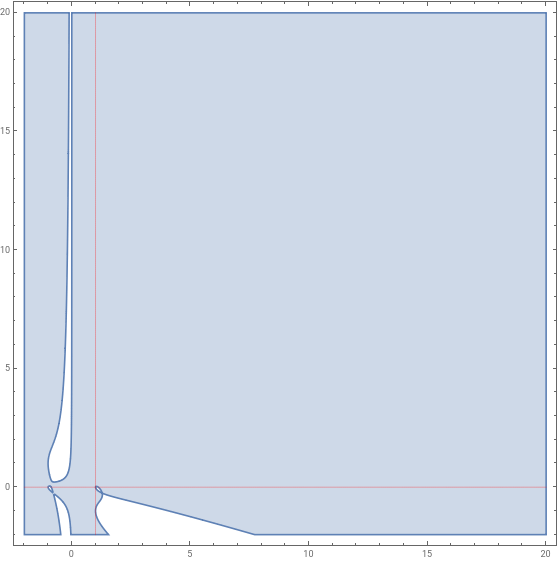
\includegraphics[width=8cm]{numeric inequality check.png}
    \caption{Numerická kontrola, že $P<1$. Osa $x$ představuje hodnoty $a$, osa $y$ zase $\alpha$. Modře je vyznačena oblast, kde nerovnost platí, červeně hranice $a=1$ a $\alpha=0$. Kontrola byla provedena pomocí metody RangePlot ve Wolfram Cloud, zkontrolováno bylo 250 bodů.}
    \label{fig:numericka_kontrola}
\end{figure}

\begin{figure}[p]
    \centering
    \begin{gnuplot}[terminal=epslatex,terminaloptions={color size 10cm, 8cm}]
        f(a,b) = (a*(a**4-1)*(1+4*b)**2) / (2*(a**2 -1 +2*a*b)**2 * (a**2 +1 +2*a*b)**2 )
        
        set ylabel "$P$"
        set xlabel "$a$"
        set yrange [0:1]
        set xrange [1:5]
        set samples 1000
        
        plot f(x, 0.04) t "$\\alpha=0.04$" lw 4, f(x, 0.2) t "$\\alpha=0.2$" lw 4, f(x, 1) t "$\\alpha=1$" lw 4, f(x, 3) t "$\\alpha=3$" lw 4
    \end{gnuplot}
    \caption{Pravděpodobnost zachycení při různých hodnotách $a, \alpha$.}
    \label{fig:grafik}
\end{figure}


\subsection*{Dodatečné poznámky}
V textu jsme o prvcích $L^2$ mluvili jako o \textit{funkcích}, požadovali po nich, aby byly spojité, a dokonce brali jejich funkční hodnoty v bodě. Situace ovšem není tak jednoduchá – prvky $L^2$ jsou ve skutečnosti třídy ekvivalence, jsou to \textit{„funkce až na rovnost skoro všude“}. Když tedy mluvíme o tom, že funkce $f\in L^2$ je spojitá na $\Omega$, myslíme tím \textit{esenciálně} spojitá – tj. že existuje takový reprezentant $\tilde f$ z třídy ekvivalence $f$, že $\tilde f \in \mathcal{C}(\Omega)$. Když potom bereme funkční hodnotu $f(x), \, x \in \Omega$, myslíme tím ve skutečnosti funkční hodnotu $\tilde f(x)$. Ve stejném smyslu bereme i funkční derivace (tj. $f'(x) \coloneqq \tilde f'(x)$), po kterých vyžadujeme, aby byly definovány pouze \textit{skoro} všude.


\end{document}
